\section{Leitungscodes, WLAN}

\begin{defi}{Basisband}
    In der Nachrichtentechnik ist das \emph{Basisband} der natürliche Frequenzbereich des Nutzsignals\footnote{untere Grenzfrequenz $f_{\min} \approx 0 \ \text{Hz}$}.

    Der belegte Frequenzbereich wird mit dem Wert der Bandbreite $B$ ausgedrückt.

    Die digitalen Informationne werden direkt in physikalische Größen übersetzt und so über die Leitung übertragen.

    Hierzu sind Kodierungsverfahren notwendig, die festlegen, wie bei der Übertragung eine 0 bzw. eine 1 repräsentiert werden.

    Es kann immer nur je ein Signal übertragen werden.
\end{defi}

\begin{defi}{Breitband}
    Die digitalen Nutzdaten werden beim \emph{Breitband} nicht direkt übertragen, sonderen einem oder mehreren hochfrequenten Trägern \enquote{aufmoduliert}.

    Durch die Verwendung verschiedener Trägerwellen (Frequenzen) können dann mehrere Informationen gleichzeitig übermittelt werden.
\end{defi}

\subsection{Leitungscodes}

\begin{defi}{Leitungscode}
    Der \emph{Leitungscode} legt bei der digitalen Telekommunikation fest, wie die zur Informationsübertragung genutzten Symbole auf der physischen Ebene übertragen werden.

    Dabei werden bestimmte Pegelfolgen, etwa Lichtintensitäten auf Glasfasern oder Spannungen oder Ströme auf elektrischen Leitungen, binären Bitsequenzen im Datenstrom zugeordnet.

    Anforderungen an einen Leitungscode sind:
    \begin{itemize}
        \item \emph{Effizienz}: möglichst hohe Übertragungsraten durch Codewörter
        \item \emph{Taktrückgewinnung} beim Empfänger (\emph{Synchronisation}): möglichst häufige bzw. regelmäßige Pegelwechsel
        \item \emph{Gleichstromfreiheit}: positive und negative Signale treten ungefähr gleich oft auf
        \item \emph{Robustheit}: Erkennen von längeren Sequenzen von 0 bzw. 1 und von fehlerhaften Bits
    \end{itemize}
\end{defi}

\begin{bonus}{Baudrate vs. Bitrate}
    Wenn die Zeitdauer (Schrittdauer) eines Symbols bzw. Codeelements $T$ ist, ist die Schrittgeschwindigkeit bzw. \emph{Baudrate}:
    \[
        v_s = \frac{1}{T} \text{ [Baud]}
    \]

    Die dazugehörige Übertragungsgeschwindigkeit bzw. \emph{Bitrate} ist dann:\footnote{$n$ = Anzahl diskreter Zustände des Codeelements}
    \[
        v_u = v_s \log_2 n
    \]

    Bei binären Codeelementen stimmen somit Bitrate und Baudrate überein, falls nur Codeelementen für Daten übermittelt werden.
\end{bonus}

\begin{defi}{NRZ-Code}
    Der \emph{NRZ-Code (Non Return to Zero)} ordnet direkt jedem Bit-Wert einen Leitungszustand zu.
    Er kann ohne weiteres verwendet werden, wenn in den Nutzdaten keine langen konstanten Folgen auftreten, wie etwa bei ASCII-kodierten Texten.

    Von Nachteil ist, dass der Empfänger bei der Übertragung einer längeren Folge gleicher Symbole unsicher wird über die Länge der Folge.

    Die NRZ-Kodierung ist im Allgemeinen auch nicht gleichanteilsfrei und damit insbesondere bei magnetischer Datenaufzeichnung problematisch.
\end{defi}

\begin{example}{NRZ-Code}
    \centering
    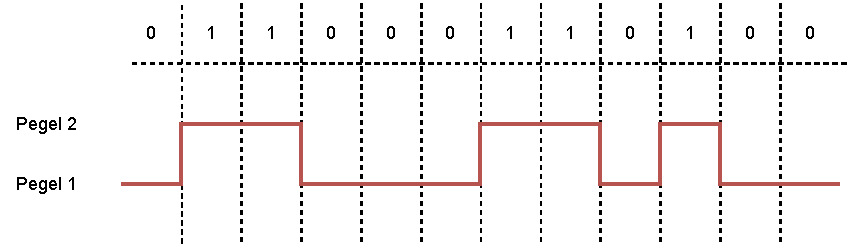
\includegraphics[width=.9\textwidth]{includes/figures/example_nrz.pdf}
\end{example}

\begin{defi}{NRZ-I-Code}
    Die \emph{NRZI-Kodierung (Non Return to Zero Inverted)} ordnet einem der beiden Bit-Werte den bereits anliegenden Leitungszustand zu, dem anderen Bit-Wert einen Zustandswechsel (Inversion).

    Daraus ergibt sich unmittelbar die Polaritätsfreiheit: Ein Verpolen der Übertragungsleitung ändert nicht die Bitfolge.
\end{defi}

\begin{example}{NRZ-I-Code}
    Im folgenden Beispiel bewirken Einsen einen Zustandswechsel.

    \centering
    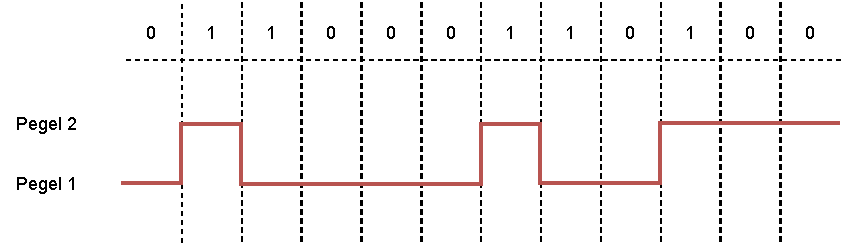
\includegraphics[width=.9\textwidth]{includes/figures/example_nrzi.pdf}
\end{example}

\begin{defi}{RZ-Code}
    Beim \emph{Return-to-Zero-Code (RZ-Code)} handelt es sich um einen Leitungscode, mit dem es möglich ist, Binärzahlen über ein Medium zu übertragen, indem der Sender dessen Zustand zwischen drei Pegelwerten (Sendesymbole, meist als +1, 0 und -1 bezeichnet) wechseln lässt.

    Dadurch gibt es beim Übertragen eines Bits garantiert eine Pegeländerung, welche der Empfänger zur Taktrückgewinnung (Synchronisierung) nutzen kann.

    Nachteilig gegenüber dem NRZ-Code ist, dass eine doppelt so große Bandbreite benötigt wird.
\end{defi}

\begin{bonus}{RZ-Code (unipolar)}
    Eine Sonderform stellt die \emph{unipolare RZ-Kodierung} dar.

    Der Vorteil besteht darin, dass nur zwei Pegelwerte (+1 und 0) als Symbole benötigt werden und diese Codierung daher mit herkömmlichen Digitalschaltungen leicht realisiert werden kann.

    Der Nachteil besteht darin, dass bei der Übertragung einer langen logisch-0-Folge, welche mit konstantem Pegel 0 codiert wird, keine Signaländerung erfolgt und damit eine Synchronisierung seitens des Empfängers unmöglich ist.
\end{bonus}

\begin{example}{RZ-Code (unipolar)}
    \centering
    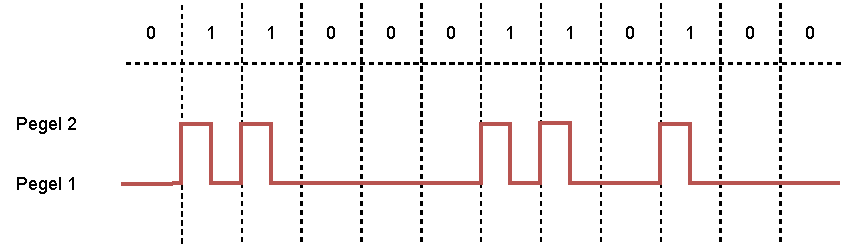
\includegraphics[width=.9\textwidth]{includes/figures/example_rz.pdf}
\end{example}

\begin{defi}{Manchester-Code}
    Der \emph{Manchester-Code} ist ein Leitungscode, der bei der Kodierung das Taktsignal erhält.

    Es gibt für den Manchester-Code zwei mögliche und gleichwertige Definitionen:
    \begin{itemize}
        \item \emph{G.E. Thomas}: eine fallende Flanke eine logische Eins, eine steigende Flanke eine logische Null.
        \item \emph{IEEE 802.3}: eine fallende Flanke eine logische Null und eine steigende Flanke eine logische Eins.
    \end{itemize}
\end{defi}

\begin{example}{Manchester-Code (G.E. Thomas)}
    \centering
    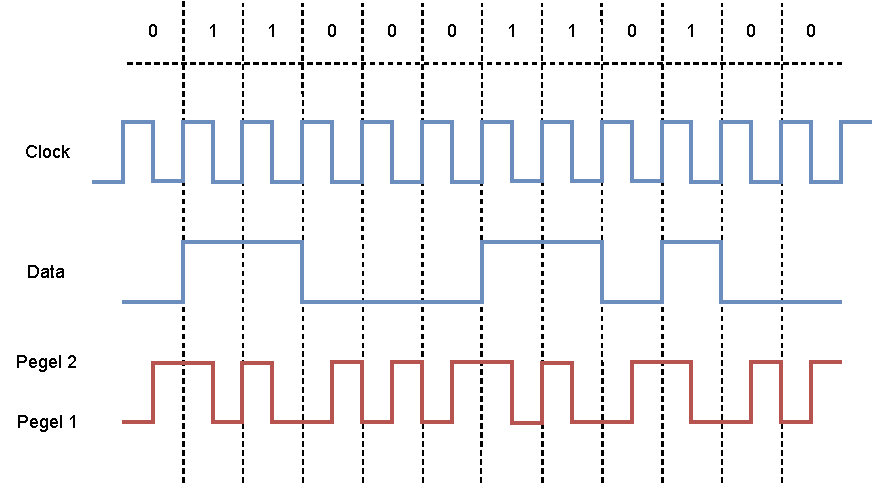
\includegraphics[width=.9\textwidth]{includes/figures/example_manchester.pdf}
\end{example}

\begin{defi}{Differentieller Manchester-Code}
    Der \emph{differentielle Manchester-Code} ist ein Leitungscode zur Übertragung von Bitfolgen als Digitalsignal.

    Wie beim Manchester-Code enthält jede Bitperiode mindestens eine Flanke, zwecks einfacher und robuster Taktrückgewinnung.
    Zusätzlich ist es invariant gegen Verpolung.

    Zusätzlich gilt:
    \begin{itemize}
        \item Eine Null bewirkt einen Pegelwechsel am Anfang des Symbols.
        \item Eine Eins bewirkt \emph{keinen} Pegelwechsel am Anfang des Symbols.
    \end{itemize}
\end{defi}

\begin{example}{Differentieller Manchester-Code}
    \centering
    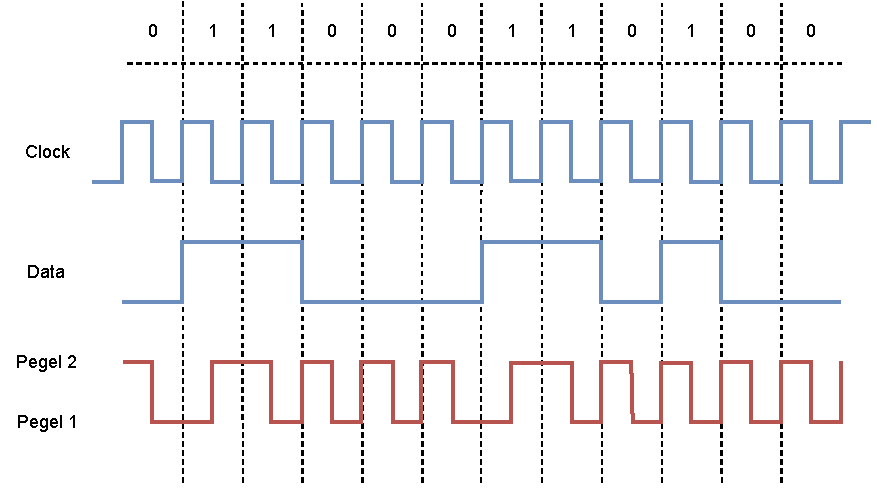
\includegraphics[width=.9\textwidth]{includes/figures/example_differentieller_manchester.pdf}
\end{example}

\begin{defi}{4B/5B-Code}
    Der \emph{4B5B-Code} beschreibt einen Leitungscode, der eindeutig umkehrbar vier Nutzdatenbits auf fünf Codebits abbildet.

    Durch das Einfügen eines weiteren Bits erhöht sich die codierte Bitrate gegenüber der Nutzdatenbitrate um 25\%.
\end{defi}

\subsection{Breitbandkommunikation}

\begin{defi}{Breitbandkommunikation}
    Bei der \emph{Breitbandkommunikation} wird das digitale Signal auf ein analoges Trägersignal aufmoduliert.

    Daten werden physikalisch als elektromagnetische Wellen dargestellt.
\end{defi}

\begin{defi}{Amplitudenmodulation}
    Bei der \emph{Amplitudenmodulation (Amplitude Shift Keying, ASK)} wird
    \begin{itemize}
        \item bei einer 1 eine große Amplitude ausgestrahlt,
        \item bei einer 0 eine kleine.
    \end{itemize}

    Die Amplitudenmodulation ist störanfällig wegen der Abschwächung der Signalstärke.
\end{defi}

\begin{example}{Amplitudenmodulation}
    \centering
    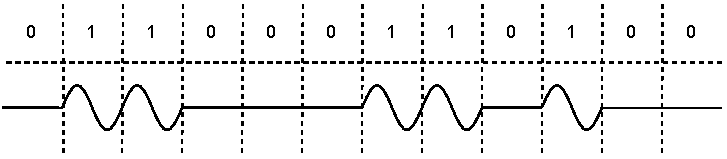
\includegraphics[width=.9\textwidth]{includes/figures/example_amplitudenmodulation.pdf}
\end{example}

\begin{defi}{Frequenzmodulation}
    Bei der \emph{Frequenzmodulation (Frequence Shift Keying, FSK)} werden für 0 und 1 verschiedene Frequenzen ausgestrahlt.

    Das Problem ist hier ein verschwenderischer Umgang mit Frequenzen.
\end{defi}

\begin{example}{Frequenzmodulation}
    \centering
    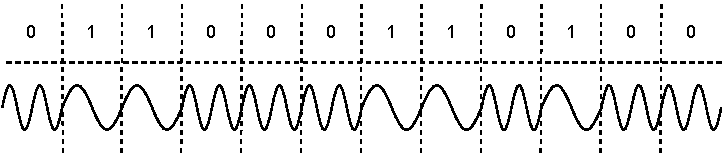
\includegraphics[width=.9\textwidth]{includes/figures/example_frequenzmodulation.pdf}
\end{example}

\begin{defi}{Phasenmodulation}
    Bei der \emph{Phasenmodulation (Phase Shift Keying, PSK)} werden für 0 und 1 verschiedene Phasenlagen verwendet.

    Das Problem ist komplexe Demodulation, allerdings ist Phasenmodulation störsicher.
\end{defi}

\begin{example}{Phasenmodulation}
    \centering
    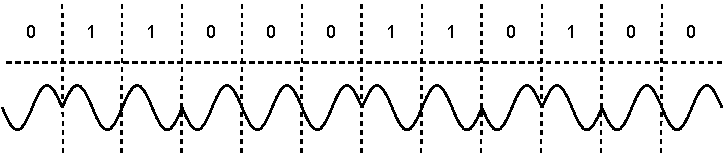
\includegraphics[width=.9\textwidth]{includes/figures/example_phasenmodulation.pdf}
\end{example}

\begin{defi}{Nyquist-Shannon-Abtasttheorem}
    Das \emph{Nyquist-Shannon-Abtasttheorem} besagt, dass ein auf $f_{\text{max}}$ bandbegrenztes Signal aus einer Folge von äquidistanten Abtastwerten exakt rekonstruiert werden kann, wenn es mit einer Frequenz von größer als $2 \cdot f_{\text{max}}$ abgetastet wurde.
\end{defi}

\subsection{WLAN}

\begin{defi}{WLAN}
    \emph{Wireless Local Area Network (WLAN)} bezeichnet ein lokales Funknetz, wobei meist ein Standard der IEEE-802.11-Familie gemeint ist.
\end{defi}

\begin{defi}{WLAN-Netze}
    WLANs können in verschiedenen Modi betrieben werden:
    \begin{itemize}
        \item \emph{Infrastruktur-Modus}:
              \begin{itemize}
                  \item ähnelt im Aufbau dem Mobilfunknetz
                  \item Wireless Access Point übernimmt Koordination aller Clients
              \end{itemize}
              \begin{center}
                  \vspace{1em}
                  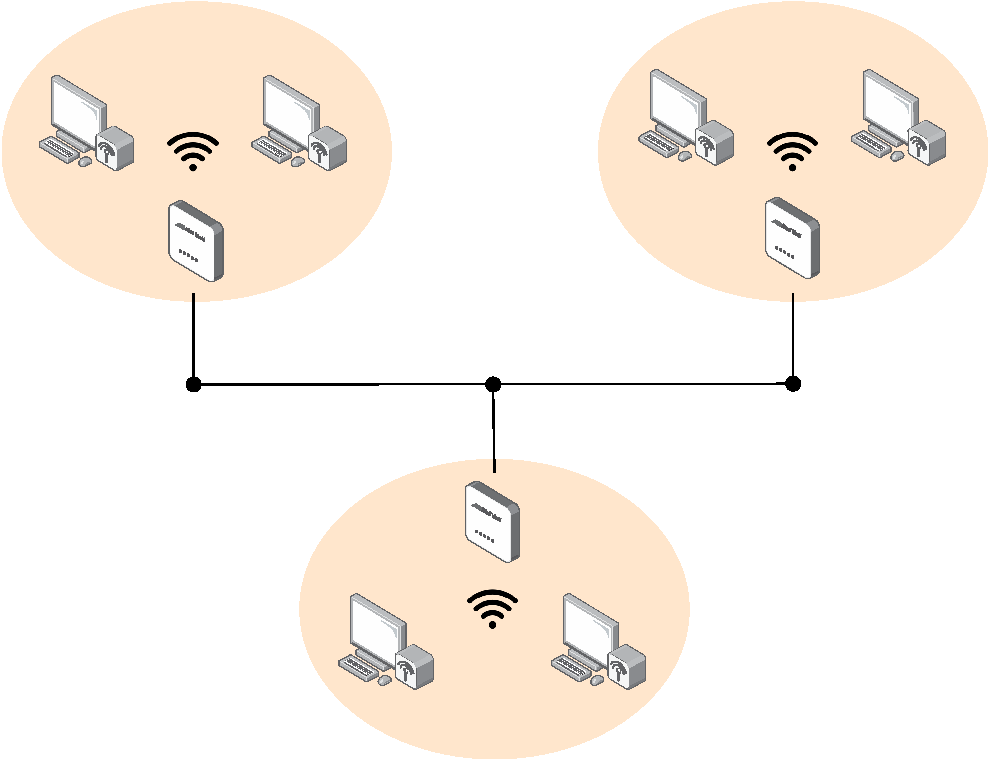
\includegraphics[width=.6\textwidth]{includes/figures/defi_wlan.pdf}
              \end{center}
        \item \emph{Ad-hoc-Modus}:
              \begin{itemize}
                  \item keine Station besonders ausgezeichnet, sondern alle sind gleichwertig
                  \item lassen sich schnell und ohne großen Aufwand aufbauen
                  \item für die spontane Vernetzung weniger Endgeräte sind allerdings andere Techniken\footnote{wie Bluetooth} eher gebräuchlich.
              \end{itemize}
              \begin{center}
                  \vspace{1em}
                  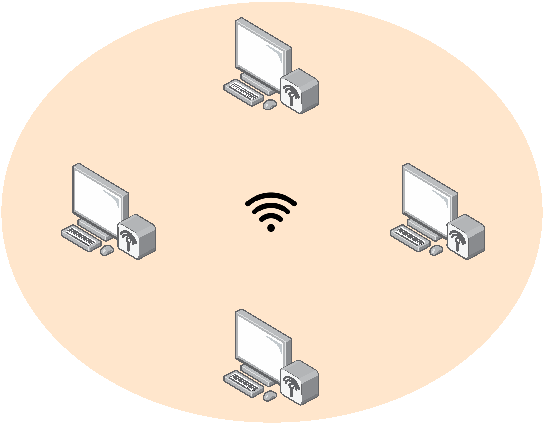
\includegraphics[width=.3\textwidth]{includes/figures/defi_adhoc.pdf}
              \end{center}
    \end{itemize}
\end{defi}

\begin{defi}{Hidden-Station-Problem}
    Eine \emph{Hidden Station} bezeichnet in asynchronen und nicht zentral koordinierten Kommunikationsnetzen, Funknetzen oder Rechnernetzen den unerwünschten Umstand, dass bei einer Übertragung zwischen zwei Teilnehmern (A und B) ein weiterer potentieller Sender (C, das Hidden Terminal) in der Nähe des Empfängers (B) ist, der vom eigentlichen Sender (A) nicht gesehen werden kann.

    Dieser potentielle Sender (C) kann die Kommunikation der anderen beiden Knoten (A und B) stören, indem er ebenfalls eine Nachricht an den Knoten in der Mitte (B) sendet, dies kann zu einer Kollision an dem Empfänger (B) führen.

    \centering
    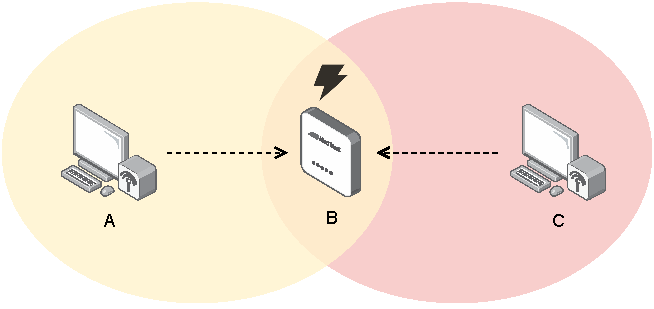
\includegraphics[width=.5\textwidth]{includes/figures/defi_hidden_station.pdf}
\end{defi}

\begin{defi}{Exposed-Station-Problem}
    Unter einer \emph{Exposed Station} versteht man, wenn eine Station B an A sendet und nun C an irgendeine andere Station senden möchte, die nicht im Sendebereich von B liegt.

    C erkennt die Signale von B und wartet, bis die Übertragung zwischen B und A vorbei ist.

    Da die Funkwellen von C aber Station A gar nicht erreichen können, wäre es gar nicht nötig zu warten: bei A könnte gar kein Konflikt auftreten.

    Dennoch ist C von der Sendung der anderen beiden Stationen abhängig (ausgeliefert).

    Durch das unnötige Warten wird Bandbreite verschwendet.

    \centering
    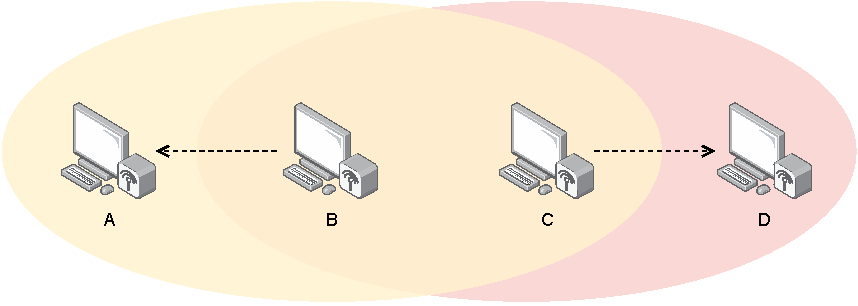
\includegraphics[width=.6\textwidth]{includes/figures/example_exposed_station.pdf}
\end{defi}

\begin{defi}{CSMA/CA}
    Der Begriff \emph{Carrier Sense Multiple Access/Collision Avoidance (CSMA/CA)} bezeichnet ein Prinzip für die Kollisionsvermeidung bei Zugriff mehrerer Netzwerkstationen auf denselben Übertragungskanal. Es wird häufig unter anderem bei drahtlosen Netzwerken (Wireless LANs) eingesetzt.

    Möchte ein Gerät Daten nach dem CSMA/CA-Verfahren versenden, so ist unter anderem folgender Ablauf möglich:
    \begin{enumerate}
        \item Zuerst wird das Medium abgehört (\emph{Carrier Sense})
        \item Ist das Medium für die Dauer eines DIFS\footnote{\emph{DIFS (Distributed Coordination Function Interframe Spacing)}: Die Zeit, die vor dem Senden eines regulären Datenframes vergangen sein muss.} frei, wird eine Backoffzeit aus dem Contention Window ausgewürfelt und nach Ablauf dieser gesendet.
        \item Ist das Medium belegt, wird der Backoff bis zum Ablauf des \emph{Network Allocation Vectors (NAV)} gestoppt, bevor er nach einem weiteren DIFS entsprechend weiter läuft.
        \item Nach vollständigem Empfang des Paketes wartet der Empfänger ein SIFS\footnote{\emph{SIFS (Short Interframe Spacing)}: Die Zeit, die vergangen sein muss vor dem Senden eines Bestätigungsframes (ACKs), eines \emph{Clear to Send}-Pakets (CTSs)}, bevor das ACK gesendet wird.
        \item Eine Kollision durch gleichzeitigen Ablauf des Backoffs führt zu einem ACK-Timeout – nach welchem ein EIFS\footnote{\emph{EIFS (Extended Interframe Spacing)}: Die Zeit, die vor dem Senden nach einer erkannten Kollision vergangen sein muss.} gewartet wird, bevor sich der gesamte Vorgang wiederholen kann
    \end{enumerate}
\end{defi}